\documentclass[11pt,letterpaper]{article}
\usepackage[lmargin=1in,rmargin=1in,tmargin=1in,bmargin=1in]{geometry}
\usepackage{../style/homework}
\usepackage{../style/commands}
\setbool{quotetype}{false} % True: Side; False: Under
\setbool{hideans}{true} % Student: True; Instructor: False

% -------------------
% Content
% -------------------
\begin{document}

\homework{20: Due 11/30}{The philosophy of the school room in one generation will be the philosophy of government in the next.}{Abraham Lincoln}

% Problem 1
\problem{10} For each of the following quadratic functions, i.e. functions which can be written as $f(x)= ax^2 + bx + c$, identify $a, b, c$:
	\begin{enumerate}[(a)]
	\item $2x^2 - 5x + 7$
	\item $6x + 9 - x^2$
	\item $x^2 - 16$
	\item $(x + 1)^2$
	\item $(x - 2)(x + 3)$
	\end{enumerate}



\newpage



% Problem 2
\problem{10} Consider the quadratic function $f(x)= 4 - (x - 2)^2$.
	\begin{enumerate}[(a)]
	\item Determine if the given parabola opens upwards or downwards.
	\item Is the parabola convex or concave?
	\item Does the function $f(x)$ have a maximum or a minimum?
	\item Find the vertex and axis of symmetry. 
	\item Find the maximum or minimum value of $f(x)$. 
	\item Sketch a graph of $f(x)$ on the plot below. 
	\end{enumerate} \vfill

	\[
	\fbox{
	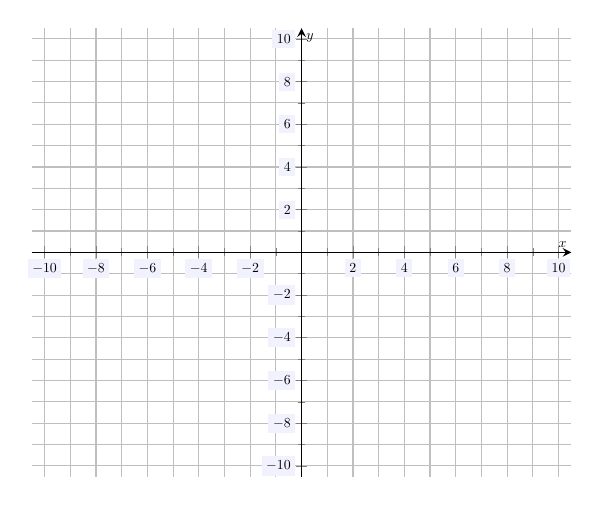
\begin{tikzpicture}[scale=1,every node/.style={scale=0.5}]
	\begin{axis}[
	grid=both,
	axis lines=middle,
	ticklabel style={fill=blue!5!white},
	xmin= -10.5, xmax=10.5,
	ymin= -10.5, ymax=10.5,
	xtick={-10,-8,-6,-4,-2,0,2,4,6,8,10},
	ytick={-10,-8,-6,-4,-2,0,2,4,6,8,10},
	minor tick = {-10,-9,...,10},
	xlabel=\(x\),ylabel=\(y\),
	]
	\end{axis}
	\end{tikzpicture}
	}
	\]



\newpage



% Problem 3
\problem{10} Showing all your work, put $f(x)= 2x^2 - 12x - 13$ into vertex form. Also, find the vertex and axis of symmetry for $f(x)$. 


\end{document}